\section{Programming and MPI skills}

Figure ~\ref{fig:Q2-Q3X} shows the results of Cross-tab analysis of “Q2: Rate your overall programming skill (non-MPI programs)” and “Q3: Rate your MPI programming skill”. The color depth represents the distribution of the answers, and the dark-colored portions represent the parts with the most answers. The vertical axis represents the Q2 answer, with lower valuesindicating higher programming skills. The horizontal axis shows the answer of Q3, and the right side shows that the MPI programming skill is high.

\begin{figure}[htb]
\begin{center}
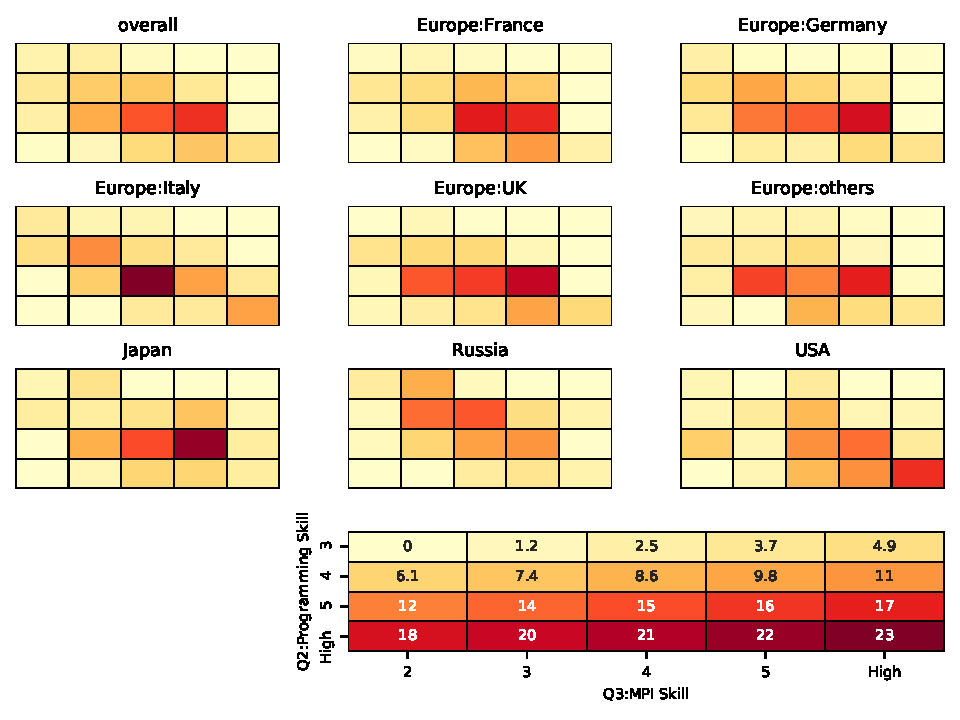
\includegraphics[width=10cm]{../pdfs/Q2-Q3.pdf}
\caption{Cross-tab analysis: Q2 and Q3}
\label{fig:Q2-Q3X}
\end{center}
\end{figure}

From Figure ~\ref{fig:Q2-Q3X} we can see:
- Because the darker colors are biased downwards as a whole, programmers who handle MPI have high programming skills of non-MPI programs.
- Because darker colors are distributed diagonally on figure, the United States has high MPI programming skills in proportion to programming skills.
- Because darker colors are distributed at the top of figure, Russia has begun MPI programming early in its learning of programming.
- Because darker colors are distributed in the middle, many people outside of the United States believe that non-MPI and MPI programming skills can be enhanced.

In order to handle MPI, programming skills of non-MPI programs need to be high because the programming model of a parallel programs are more complicated than the sequential program. It is difficult to write a program that is conscious of parallel execution from the beginning, and even if MPI prepare a simple MPI API, this problem will not be solved. However, even if the problem is not solved, in order for more people to achieve higher results by using parallel execution more widely, it is necessary to have an interface that can be easily programmed like a sequential program.

In the United States, as a result of introducing MPI programming education according to programming skills, people have acquired MPI programming skills that correspond to their programming skills. When learning something, teaching materials are an important element, but since many of the teaching materials are written in English. Compared to a country where English is not the native language, the environment for learning MPI programming for English native speakers are more blessed with more information on MPI programming.

On the other hand, in Russia, there are currently few people who can master MPI, but it turns out that programmers who do not have high programming skills are challenging MPI programming. This indicates that they are is teaching parallel programming since they have little programming experience. The effect of the education can be confirmed by observing the result when a similar survey is taken several years later.

Other than the United States, few people position themselves as highly skilled non-MPI and MPI programmers. We analyze this because they still feel that they don't know everything about MPI. As it can be seen from Q9 which is the question “Have you ever read the MPI standard speciation document?”, nearly 85\% of the people who actually read the entire specification document, they knew that there were some functions that they did not know yet because they read only the necessary parts of the MPI standard speciation document. The result may change if information that can be easily overviewed is prepared to understand what functions MPI has.

By analyzing the relationship between non-MPI programming skills and MPI programming skills, it is possible to see what efforts are necessary to spread MPI.

